%%%%%%%%%%%%%%%%%%%%
%%%%%%%%%%%%%%%%%%%%

\begin{frame}
%    \shiftedframetitle{2. Theory}
%\begin{itemize}
%\item NS discussion
%\item SWE derivation
%\end{itemize}
    \shiftedframetitle{2. Theory\\[0.3cm]{\large Shallow Water Equations (SWE) model {\small  (initial)}}}

%\vspace{-3mm}
\begin{minipage}{0.35\textwidth}
\begin{itemize}
\item<1->[]
\begin{align*}
\frac{\partial u}{\partial x} + \frac{\partial v}{\partial y} + \frac{\partial w}{\partial z} &= 0
\end{align*}
\item<1->[]
\begin{align*}
\frac{\partial u}{\partial t} + u\frac{\partial u}{\partial x} + v\frac{\partial u}{\partial y} + w\frac{\partial u}{\partial z} &= - \frac{\partial p}{\partial x}
\end{align*}
\item<1->[]
\begin{align*}
\frac{\partial v}{\partial t} + u\frac{\partial v}{\partial x} + v\frac{\partial v}{\partial y} + w\frac{\partial v}{\partial z}&= - \frac{\partial p}{\partial y}
\end{align*}
\item<1->[]
\begin{align*}
\frac{\partial w}{\partial t} + u\frac{\partial w}{\partial x} + v\frac{\partial w}{\partial y} + w\frac{\partial w}{\partial z} &= - \frac{\partial p}{\partial z} + g \end{align*}
\end{itemize}
\end{minipage}
\hspace{1.5cm}
\begin{minipage}{0.35\textwidth}
\includegraphics[scale=0.65]{./Resources/Images/imagesThesis/floor.png}%
\end{minipage}
\end{frame}
\clearpage

%%%%%%%%%%%%%%%%%%%%
%%%%%%%%%%%%%%%%%%%%

\begin{frame}
    \shiftedframetitle{2. Theory\\[0.3cm]{\large Shallow Water Equations (SWE) model {\small  (initial)}}}
\begin{minipage}{0.35\textwidth}
\begin{itemize}
\item<1->[]
\begin{align*}
\color{TUMOrange}\underbrace{\color{black}\frac{\partial u}{\partial x} + \frac{\partial v}{\partial y}}_{\approx \frac{2U}{L}} \color{black} + \color{TUMOrange}\underbrace{\color{black}\frac{\partial w}{\partial z}}_{\myTUMorange{\approx \frac{W}{H}}} &= 0
\end{align*}
\item<1->[]
\begin{align*}
\frac{\partial u}{\partial t} + u\frac{\partial u}{\partial x} + v\frac{\partial u}{\partial y} + w\frac{\partial u}{\partial z} &= - \frac{\partial p}{\partial x}
\end{align*}
\item<1->[]
\begin{align*}
\frac{\partial v}{\partial t} + u\frac{\partial v}{\partial x} + v\frac{\partial v}{\partial y} + w\frac{\partial v}{\partial z}&= - \frac{\partial p}{\partial y}
\end{align*}
\item<1->[]
\begin{align*}
\color{TUMDarkBlue}\underbrace{\color{black}\frac{\partial w}{\partial t} + u\frac{\partial w}{\partial x} + v\frac{\partial w}{\partial y} + w\frac{\partial w}{\partial z}}_{\myTUMdarkblue{0}}  \color{black} = - \frac{\partial p}{\partial z} + g
%\myTUMdarkblue{0} \myTUMdarkblue{= - \frac{\partial p}{\partial z} + g}
\end{align*}
\end{itemize}
\end{minipage}
\hspace{0.5cm}
\begin{minipage}{0.15\textwidth}
\begin{itemize}
\item<2->[]
%
\includegraphics[width=1\textwidth]{Resources/Images/download.png}\\[2cm]

\includegraphics[width=1\textwidth]{Resources/Images/arrow.png}\\
\item<3->[] {\LARGE  \makebox[\textwidth]{+}}
\item<3->[] {\Large \makebox[\textwidth]{\myCRed{Depth-Averaged}}}
\item<3->[] {\Large \makebox[\textwidth]{\myCRed{integration}}}
\end{itemize}
\end{minipage}
\hspace{1cm}
\begin{minipage}{0.4\textwidth}
\begin{itemize}
\item<2->[]
\begin{align*}
\myTUMdarkblue{0} \myTUMdarkblue{= - \frac{\partial p}{\partial z} + g}
\end{align*}
\item<3->[]
\begin{tcolorbox}
\begin{align*}
\myCRed{\frac{\partial h}{\partial t}} + \frac{\partial \myCRed{h}u}{\partial x} + \frac{\partial \myCRed{h}v}{\partial y} &= 0\\[0.5cm]
\frac{\partial \myCRed{hu}}{\partial t} + \frac{\partial}{\partial x}(\myCRed{hu^2} + \myTUMdarkblue{\frac{1}{2} g h^2}) + \frac{\partial \myCRed{huv}}{\partial y} &= \myTUMdarkblue{- gh\frac{\partial b}{\partial x}} \\[0.5cm]
\frac{\partial \myCRed{hv}}{\partial t} + \frac{\partial \myCRed{huv}}{\partial x} + \frac{\partial}{\partial y}(\myCRed{hv^2} + \myTUMdarkblue{\frac{1}{2} g h^2})&= \myTUMdarkblue{- gh\frac{\partial b}{\partial y} }
\end{align*}
\end{tcolorbox}
\end{itemize}
\end{minipage}
\end{frame}
\clearpage

%%%%%%%%%%%%%%%%%%%%%
%%%%%%%%%%%%%%%%%%%%%
%
%\begin{frame}
%    \shiftedframetitle{\large Shallow Water Equations (SWE) model {\small (cont.)}}
%\vspace{-3mm}
%\begin{itemize}
%\setlength\itemsep{2em}
%\item<1-> \textbf{First assumption}: $L \gg H$, from mass continuity (\ref{cont})
%\begin{align*}
%\color{TUMOrange}\underbrace{\color{black}\frac{\partial u}{\partial x} + \frac{\partial v}{\partial y}}_{\approx \frac{2U}{L}} \color{black} + \color{TUMOrange}\underbrace{\color{black}\frac{\partial w}{\partial z}}_{\myTUMorange{\approx \frac{W}{H}}} &= 0
%\end{align*}
%
%leading to \myTUMorange{$u,v\gg w$}
%\item<2-> \textbf{Second assumption}: \myTUMdarkblue{vertical momentum exchange} is \myTUMdarkblue{negligible}. Then, NS equation \myTUMdarkblue{vertical component} modifies to
%\begin{align}
%\color{TUMDarkBlue}\underbrace{\color{black}\frac{\partial w}{\partial t} + u\frac{\partial w}{\partial x} + v\frac{\partial w}{\partial y} + w\frac{\partial w}{\partial z}}_{\myTUMdarkblue{0}}  \color{black} = - \frac{\partial p}{\partial z} + g \nonumber\\[0.5cm]
%\myTUMdarkblue{0} \myTUMdarkblue{= - \frac{\partial p}{\partial z} + g} \label{press}
%\end{align}
%\item<3->[]
%This provides a \myTUMdarkblue{solution for the pressure} as a function of the sea floor elevation and water level
%\end{itemize}
%\end{frame}
%\clearpage
%


%%%%%%%%%%%%%%%%%%%%%
%%%%%%%%%%%%%%%%%%%%%
%\begin{frame}
%    \shiftedframetitle{\large Shallow Water Equations (SWE) model {\small(cont.)}}
%\vspace{-3mm}
%\begin{itemize}
%\item<1-> \myTUMorange{Depth-averaged integration} on the continuity equation \ref{cont}
%\begin{align}
%\myTUMorange{\int_{b_0}^{b_0 + h }} (\frac{\partial u}{\partial x} + \frac{\partial v}{\partial y} + \myTUMorange{\frac{\partial w}{\partial z}})\ \myTUMorange{dz} &= 0 \nonumber \\[0.8cm]
%\myTUMorange{\frac{\partial h}{\partial t}} + \frac{\partial \myTUMorange{h}u}{\partial x} + \frac{\partial \myTUMorange{h}v}{\partial y} &= 0
%\end{align}
%\vspace{0.5cm}
%\item<2->\myCRed{\textit{Leibnitz Integral Rule}} $+$ \myCRed{depth-averaged integration} on the momentum equation $+$ kinematic \myCRed{BCs} on surface \cite{depthAv} $+$ \myTUMdarkblue{(\ref{press})}
%\begin{align}
%\frac{\partial \myCRed{hu}}{\partial t} + \frac{\partial}{\partial x}(\myCRed{hu^2} + \myTUMdarkblue{\frac{1}{2} g h^2}) + \frac{\partial \myCRed{huv}}{\partial y} &= \myTUMdarkblue{- gh\frac{\partial b}{\partial x}} \\[0.8cm]
%\frac{\partial \myCRed{hv}}{\partial t} + \frac{\partial \myCRed{huv}}{\partial x} + \frac{\partial}{\partial y}(\myCRed{hv^2} + \myTUMdarkblue{\frac{1}{2} g h^2})&= \myTUMdarkblue{- gh\frac{\partial b}{\partial y} }
%\end{align}
%\end{itemize}
%\end{frame}
%\clearpage

%%%%%%%%%%%%%%%%%%%%
%%%%%%%%%%%%%%%%%%%%
\begin{frame}
    \shiftedframetitle{\large Shallow Water Equations (SWE) model {\small(cont)}}
%\vspace{-2mm}
%\begin{columns}
\begin{minipage}{0.35\textwidth}
\begin{itemize}
\item<1->[] SWE model can be represented in a {\color{TUMBlauDunkel}matrix} form \dots
% derived from mass and momentum conservation laws, and depth averaging \dots %also derived by vertical averaging from the 3d incompressible ns eqs
\item<1->[]
\begin{align*}
\vspace{-15pt}
\begin{bmatrix}[1.3]
\myTUMdarkblue{h}\\
\myTUMdarkblue{hu}\\
\myTUMdarkblue{hv}\\
\end{bmatrix}_t \ + \
\begin{bmatrix}[1.0]
hu\\
hu^2 + \frac{1}{2}gh^2\\
huv\\
\end{bmatrix}_x\ &+ \
\begin{bmatrix}[1.0]
hv\\
huv\\
hv^2 + \frac{1}{2}gh^2\\
\end{bmatrix}_y =
\begin{bmatrix}[1.0]
0\\
-gh\ b_x\\
-gh\ b_y
\end{bmatrix}\\[2em]
\bar{q} = &\begin{bmatrix}[1.3]
\myTUMdarkblue{h}\\
\myTUMdarkblue{hu}\\
\myTUMdarkblue{hv}
\end{bmatrix}
\begin{matrix}[1.0]
\text{\hspace{-3em}\myTUMdarkblue{$\rightarrow\ $\textit{height}}}\\
\text{\hspace{-2pt}\myTUMdarkblue{$\rightarrow\ $\textit{dicharge in x}}} \\
\text{\hspace{5pt}\myTUMdarkblue{$\rightarrow\ $\textit{discharge in y}}}
\end{matrix}
\end{align*}
\item<2->[]
\begin{align*}
\qquad \qquad \frac{\partial \bar{q}}{\partial t} + \dfrac{\partial \bar{F}(q)}{\partial x} + &\frac{\partial \bar{G}(q)}{\partial y} = S(h,x,y,t)
\end{align*}
\end{itemize}
\end{minipage}
\begin{minipage}{0.45\textwidth}  
\begin{itemize}[leftmargin=*]
\item<1->[]
\vspace{2cm}
\begin{center}
\begin{figure}
\includegraphics[scale=0.55]{./Resources/Images/imagesThesis/floor.png}%
\caption{SWE variables schematic}
\label{fig:swechemedit}
\end{figure}
\end{center}
\end{itemize}
\end{minipage}
%\end{columns}

\end{frame}
\clearpage


%%%%%%%%%%
%%%%%%%%%%
%
%\begin{frame}
%    \shiftedframetitle{Shallow Water Equations (SWE) model {\small(cont)}}
%\vspace{-2mm}
%\begin{multicols}{2}
%\begin{itemize}
%\item<1->[] SWE model can be represented in a {\color{TUMBlauDunkel}matrix} form \dots
%% derived from mass and momentum conservation laws, and depth averaging \dots %also derived by vertical averaging from the 3d incompressible ns eqs
%\item<2->[]
%\begin{align*}
%\vspace{-15pt}
%\begin{bmatrix}[1.3]
%\myTUMdarkblue{h}\\
%\myTUMdarkblue{hu}\\
%\myTUMdarkblue{hv}\\
%\end{bmatrix}_t \ + \
%\begin{bmatrix}[1.0]
%hu\\
%hu^2 + \frac{1}{2}gh^2\\
%huv\\
%\end{bmatrix}_x\ &+ \
%\begin{bmatrix}[1.0]
%hv\\
%huv\\
%hv^2 + \frac{1}{2}gh^2\\
%\end{bmatrix}_y =
%\begin{bmatrix}[1.0]
%0\\
%-gh\ b_x\\
%-gh\ b_y
%\end{bmatrix}\\[1em]
%\bar{q} = &\begin{bmatrix}[1.3]
%\myTUMdarkblue{h}\\
%\myTUMdarkblue{hu}\\
%\myTUMdarkblue{hv}\\
%\end{bmatrix}
%\begin{matrix}[1.0]
%\text{\hspace{-3em}\myTUMdarkblue{$\rightarrow\ $\textit{height}}}\\
%\text{\hspace{-2pt}\myTUMdarkblue{$\rightarrow\ $\textit{dicharge in x}}} \\
%\text{\hspace{5pt}\myTUMdarkblue{$\rightarrow\ $\textit{discharge in y}}}
%\end{matrix}\\[2em]
%\frac{\partial \bar{q}}{\partial t} + \dfrac{\partial \bar{F}(q)}{\partial x} + &\frac{\partial \bar{G}(q)}{\partial y} = S(h,x,y,t) \\[3em]
%\end{align*}
%%\end{itemize}
%
%\vfill\columnbreak
%\vspace*{0.4cm}
%%\begin{itemize}
%\item<3->[]
%\begin{figure}
%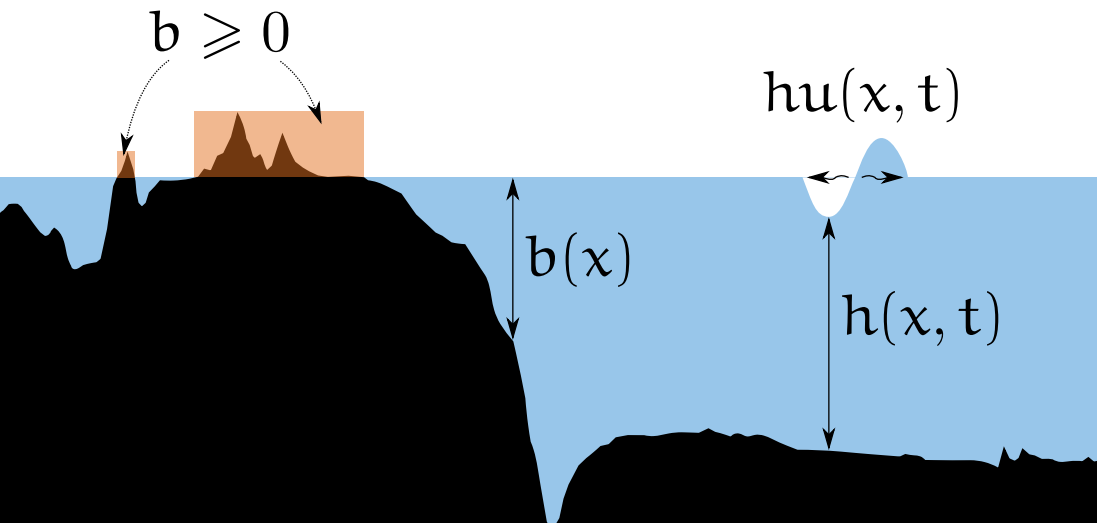
\includegraphics[scale=0.32]{./Resources/Images/swe_edit.png}%
%\caption{SWE variables schematic \footnote{\url{https://www5.in.tum.de/SWE/lugano2013/swe_anatomy.pdf}}}
%\label{fig:swechem}
%\end{figure}
%\end{itemize}
%\end{multicols}
%\end{frame}
%\clearpage

%%%%%%%%%%%%%%%%%%%%
%%%%%%%%%%%%%%%%%%%
\begin{frame}
    \shiftedframetitle{\large Shallow Water Equations (SWE) model {\small(final)}}
\hspace{3.5cm}
\begin{minipage}{0.7\textwidth}
\begin{tcolorbox}[colframe=TUMGreen,
colback=TUMGreen!30]     
\begin{itemize}
\setlength\itemsep{1.9em}
\item<1->[] The \textbf{\myTUMdarkblue{Shallow Water Equations}} \dots
\item<1-> simplify \myTUMdarkblue{$3D$} Navier-Stokes \myTUMdarkblue{to} a \myTUMdarkblue{$2D$} system of equations
\item<1-> \myTUMdarkblue{neglect vertical velocity}:  $ W \ll U,V $, horizontal distances $L$ $\gg$ vertical distance $H$
\item<1-> represent a \myTUMdarkblue{hyperbolic PDE} system $\rightarrow$ \myTUMdarkblue{Riemann} Problem and \myTUMdarkblue{FVM}
\item<1-> Applications: 
\begin{itemize}
\addtolength{\itemindent}{1cm}
\item \myTUMdarkblue{Free surface flows} around structures, 
\item \myTUMdarkblue{tsunamis} prediction,
\item \myTUMdarkblue{atmospheric flows}, \dots
\end{itemize}
\end{itemize}
\end{tcolorbox}
\addtolength{\leftmargini}{-0.8cm}
\begin{itemize}
\item<2->[]
\begin{tcolorbox}[colframe=TUMOrange,
colback=TUMOrange!30] 
Both NS and SWE reach a solution for free-surface problems $\rightarrow$ compatibility between the respective solution methods
\end{tcolorbox}
\end{itemize}
\end{minipage}
\end{frame}
\clearpage




%%%%%%%%%%%%%%%%%
%%%%%%%%%%%%%%%%%
\begin{frame}
    \shiftedframetitle{\large Flow characterization}
\hspace{1cm}
\begin{minipage}{0.4\textwidth}
\centering
\begin{tcolorbox}[title=\centering \textbf{Subcritical flow }, colframe=TUMDarkBlue,
colback=TUMDarkBlue!30] 
hola
\end{tcolorbox}
\vspace{0.5cm}
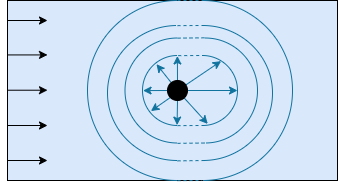
\includegraphics[width=0.8\textwidth]{Resources/Images/subcritical.png}
\end{minipage}
\hspace{1cm}
\begin{minipage}{0.4\textwidth}
\centering
\begin{tcolorbox}[title=\centering \textbf{Supercritical flow}, colframe=TUMDarkBlue,
colback=TUMDarkBlue!30] 
hola
\end{tcolorbox}
\vspace{0.5cm}
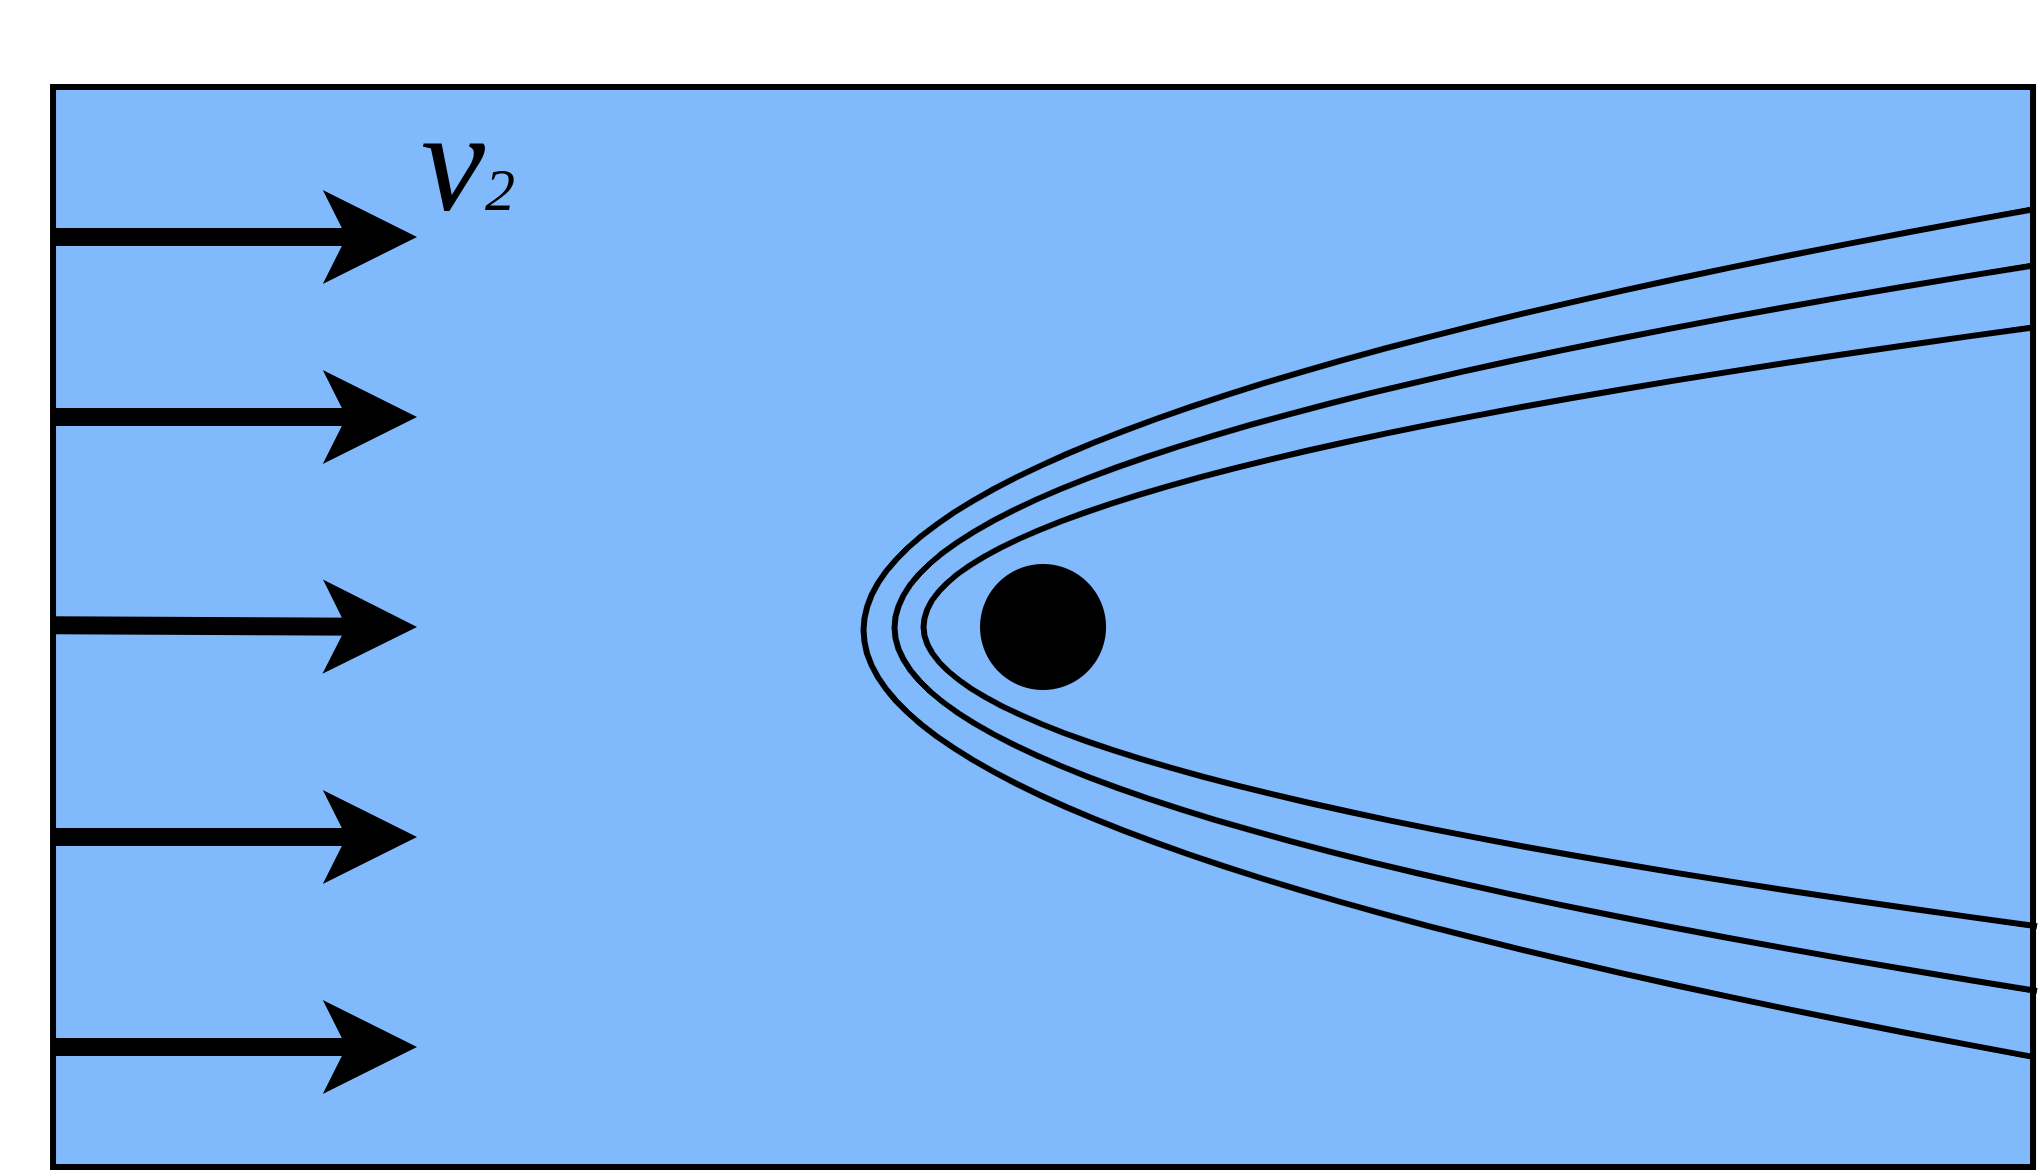
\includegraphics[width=0.8\textwidth]{Resources/Images/supercritical.png}
\end{minipage}
\end{frame}

\clearpage



\begin{frame}
    \shiftedframetitle{\large Flow characterization \small(cont)}

\begin{minipage}{0.5\textwidth}
\vspace{1cm}
\includegraphics[width=\textwidth]{Resources/Images/imagesThesis/hydjump.png}
\end{minipage}
\hspace{1cm}
\begin{minipage}{0.4\textwidth}
\begin{tcolorbox}[title=\centering \textbf{Hydraulic jump}, colframe=TUMDarkBlue,
colback=TUMDarkBlue!30] 
hola
\end{tcolorbox}
\end{minipage}
\end{frame}
